% --------------------------------------------------------------- %
% Heart Protectors - Final Report
% --------------------------------------------------------------- %
\documentclass[11pt,a4paper]{article}
\usepackage{xcolor}
\usepackage{graphicx}
\usepackage{amsmath}
\usepackage{amssymb}
\usepackage{enumitem}
\usepackage{algorithm}
\usepackage{algpseudocode}
\usepackage{etoolbox}
\AtBeginEnvironment{algorithm}{\footnotesize}
\AtBeginEnvironment{algorithmic}{\footnotesize}
\usepackage{booktabs}
\usepackage{tikz}
\usepackage[most]{tcolorbox} % Add 'most' option to load all features
\usepackage{caption}
\usepackage[top=2.5cm, bottom=2.5cm, left=2.5cm, right=2.5cm]{geometry}
\usepackage{fancyhdr}
\usepackage{setspace}
\usepackage{abstract}
\usepackage{titlesec}
\usepackage{hyperref}
\usepackage{listings}
\usepackage{float}
\usepackage{pifont} % Required for checkmark
\usepackage[export]{adjustbox}  % gives \includegraphics the roundcorner key

% Fix header height
\setlength{\headheight}{14pt}

% Highlighting
\definecolor{lightyellow}{rgb}{1,1,0.8}
\newcommand{\highlight}[1]{\colorbox{lightyellow}{$\displaystyle #1$}}

% Define green checkmark
\newcommand{\greencheck}{\textcolor{green}{\ding{52}}}

% Colors
\definecolor{lightblue}{rgb}{0.85,0.90,0.95}
\definecolor{mediumblue}{rgb}{0.70,0.80,0.90}
\definecolor{darkblue}{rgb}{0.20,0.40,0.65}
\definecolor{lightgreen}{rgb}{0.85,0.95,0.85}
\definecolor{mediumgreen}{rgb}{0.70,0.85,0.70}
\definecolor{darkgreen}{rgb}{0.20,0.65,0.40}
\definecolor{lightpurple}{rgb}{0.90,0.85,0.95}
\definecolor{mediumpurple}{rgb}{0.80,0.70,0.85}
\definecolor{lightgray}{rgb}{0.95,0.95,0.95}
\definecolor{mediumgray}{rgb}{0.85,0.85,0.85}

% Code listing style - Changed to Python
\lstset{
    language=Python,
    breaklines=true,
    basicstyle=\ttfamily\footnotesize,
    keywordstyle=\color{blue},
    identifierstyle=\color{black},
    commentstyle=\color[rgb]{0.133,0.545,0.133},
    stringstyle=\color{red},
    tabsize=4,
    showspaces=false,
    showstringspaces=false,
    numbers=left,
    numberstyle=\tiny\color{gray},
    frame=single,
    backgroundcolor=\color{lightgray},
    escapeinside={(*@}{@*)}
}

% Custom environment for consistent indentation
\newenvironment{indented}
  {\begin{list}{}{\leftmargin=1em \rightmargin=1em}\item[]}
  {\end{list}}

% Format settings
\onehalfspacing
\setlength{\parindent}{0pt}
\setlength{\parskip}{6pt}

% Title setup - improved compact version
\makeatletter
\renewcommand{\maketitle}{
  \begin{center}
    \vspace*{-0.25in} % Reduce top space
    {\LARGE \textbf{\@title}} \\[0.3cm]
    {\large \@subtitle} \\[0.2cm]
    {\normalsize \textit{\@author}} \\[0.1cm]
    {\normalsize \@date} \\
  \end{center}
  \vspace{0.3cm} % Space after title block
}
\makeatother

% Add subtitle command
\newcommand{\subtitle}[1]{\def\@subtitle{#1}}
\def\@subtitle{}

% Fancy headers
\pagestyle{fancy}
\fancyhf{}
\fancyhead[L]{Heart Failure Risk Prediction Project}
\fancyhead[R]{Team Heart Protectors - Final Report}
\fancyfoot[C]{\thepage}

% Section formatting - reduce space after section titles
\titleformat{\section}{\normalfont\large\bfseries}{\thesection}{1em}{}
\titlespacing*{\section}{0pt}{12pt}{3pt} % Reduced space after section title from default

% Subsection formatting - reduce space after subsection titles
\titleformat{\subsection}{\normalfont\normalsize\bfseries}{\thesubsection}{1em}{}
\titlespacing*{\subsection}{0pt}{12pt}{3pt} % Reduced space after subsection title

% Simpler tcolorbox styles
\tcbset{
  infobox/.style={
    colback=lightblue!30,
    colframe=darkblue,
    fonttitle=\bfseries\sffamily,
    boxrule=0.5pt,
    title=#1
  }
}

\tcbset{
  notebox/.style={
    colback=lightgreen!30,
    colframe=darkgreen,
    fonttitle=\bfseries\sffamily,
    boxrule=0.5pt,
    title=#1
  }
}

% Begin document
\begin{document}

% Add project cover image at the top
\begin{figure}[H]
    \centering
    
\includegraphics[width=0.5\textwidth]{./pictures/cover.png}
\end{figure}




% Set title, subtitle, author, and date
\title{Heart Failure Risk Prediction Using Ma chine Learning Techniques}
\subtitle{Team Meeting Report – Final Report}
\author{Team Heart Protectors}
\date{April 23, 2025}

% \maketitle
% \vspace*{-0.2in}

\begin{tabular}{ll}
    \textbf{Team Name:}         & Heart Protectors    \\
    \textbf{Team Leader:}       & Thien Van Ky Nguyen \\
    \textbf{Team Members:}      & ?, ?, ?, ?          \\
    \textbf{Meeting Date/Time:} & April 23, 2025      \\
    \textbf{Attendees:}         & All team members
\end{tabular}

\section{Project Topic / Service Scenario}

\textbf{Abstract:} Our project implements advanced machine learning techniques to predict heart failure
risk based on comprehensive health data.
Cardiovascular disease remains one of the leading causes of mortality worldwide,
with heart failure affecting millions of patients and placing significant
burden on healthcare systems.
Traditional diagnostic approaches often fail to identify
at-risk individuals until symptoms become severe,
resulting in delayed intervention and poorer outcomes.

We propose a predictive analytics framework that identifies high-risk
individuals through analysis of clinical and demographic data.
This system employs supervised learning algorithms to generate risk
assessments that could enable clinicians to implement early preventive measures.
By facilitating timely intervention, our approach has the potential to
reduce heart failure incidence, improve patient outcomes, and optimize healthcare resource allocation.

% The system uses machine learning to analyze
% health data and calculate risk scores that
% doctors could use alongside their regular patient information systems.

\section{Selected Dataset}

\begin{tcolorbox}[notebox={Dataset Information}]
    For this project, we utilize a single, comprehensive heart disease dataset from Kaggle to build and validate our predictive models:
    \vspace{-0.25cm}
    \begin{enumerate}[leftmargin=*, itemsep=2pt, parsep=0pt]
        \item \textbf{Heart Disease UCI} (10,000 entries) –
              \url{https://www.kaggle.com/datasets/oktayrdeki/heart-disease}
    \end{enumerate}
\end{tcolorbox}

\begin{table}[H]
    \centering
    \caption{Features Overview with Summary Statistics (Numerical Only)}
    \small
    \begin{tabular}{|l|l|r|r|r|r|r|}
        \hline
        \textbf{Feature}     & \textbf{Type} & \textbf{Mean} & \textbf{Std Dev} & \textbf{Min} & \textbf{Median} & \textbf{Max} \\
        \hline
        Gender               & Categorical   &               &                  &              &                 &              \\
        Exercise Habits      & Categorical   &               &                  &              &                 &              \\
        Smoking              & Categorical   &               &                  &              &                 &              \\
        Family Heart Disease & Categorical   &               &                  &              &                 &              \\
        Diabetes             & Categorical   &               &                  &              &                 &              \\
        High Blood Pressure  & Categorical   &               &                  &              &                 &              \\
        Low HDL Cholesterol  & Categorical   &               &                  &              &                 &              \\
        High LDL Cholesterol & Categorical   &               &                  &              &                 &              \\
        Stress Level         & Categorical   &               &                  &              &                 &              \\
        Sugar Consumption    & Categorical   &               &                  &              &                 &              \\
        Age                  & Numerical     & 49.30         & 18.19            & 18.00        & 49.00           & 80.00        \\
        Blood Pressure       & Numerical     & 149.76        & 17.57            & 120.00       & 150.00          & 180.00       \\
        Cholesterol Level    & Numerical     & 225.43        & 43.58            & 150.00       & 226.00          & 300.00       \\
        BMI                  & Numerical     & 29.08         & 6.31             & 18.00        & 29.08           & 40.00        \\
        Sleep Hours          & Numerical     & 6.99          & 1.75             & 4.00         & 7.00            & 10.00        \\
        Triglyceride Level   & Numerical     & 250.73        & 87.07            & 100.00       & 250.00          & 400.00       \\
        Fasting Blood Sugar  & Numerical     & 120.14        & 23.58            & 80.00        & 120.00          & 160.00       \\
        CRP Level            & Numerical     & 7.47          & 4.34             & 0.00         & 7.47            & 15.00        \\
        Homocysteine Level   & Numerical     & 12.46         & 4.32             & 5.00         & 12.41           & 20.00        \\
        \hline
    \end{tabular}
\end{table}


\section{Problems and Challenges}
% Throughout the development of our heart failure risk prediction system,
% we encountered various technical and methodological challenges
% that required careful consideration and innovative solutions.


\subsection{Data Quality and Preprocessing Challenges}

\begin{tcolorbox}[
        title=Data Quality Issues Overview,
        colback=lightpurple!30,
        colframe=mediumpurple,
        boxrule=0.5pt,
        fonttitle=\bfseries\sffamily\footnotesize,
        fontupper=\footnotesize
    ]
    Our initial analysis of the Heart Disease UCI dataset revealed:
    \begin{itemize}[leftmargin=*, itemsep=2pt, parsep=0pt]
        \item Missing values in most columns (19-30 entries per column)
        \item Significant missing data in 'Alcohol Consumption' (2,586 of 10,000 entries missing)
        \item Mix of numerical features (9) and categorical features (12)
        \item Need for proper data type conversion and standardization
    \end{itemize}

    \textbf{Missing Values by Column:}

    \begin{tabular}{lr|lr}
        Age                  & 29 & High Blood Pressure  & 26    \\
        Gender               & 19 & Low HDL Cholesterol  & 25    \\
        Blood Pressure       & 19 & High LDL Cholesterol & 26    \\
        Cholesterol Level    & 30 & Alcohol Consumption  & 2,586 \\
        Exercise Habits      & 25 & Stress Level         & 22    \\
        Smoking              & 25 & Sleep Hours          & 25    \\
        Family Heart Disease & 21 & Sugar Consumption    & 30    \\
        Diabetes             & 30 & Triglyceride Level   & 26    \\
        BMI                  & 22 & Fasting Blood Sugar  & 22    \\
                             &    & CRP Level            & 26    \\
                             &    & Homocysteine Level   & 20    \\
    \end{tabular}
\end{tcolorbox}

% NOTE:combined with the table above
% \begin{table}[H]
%     \centering
%     \caption{Summary Statistics for Key Numerical Features}
%     \small
%     \begin{tabular}{|l|r|r|r|r|r|}
%         \hline
%         \textbf{Feature}    & \textbf{Mean} & \textbf{Std Dev} & \textbf{Min} & \textbf{Median} & \textbf{Max} \\
%         \hline
%         Age                 & 49.30         & 18.19            & 18.00        & 49.00           & 80.00        \\
%         Blood Pressure      & 149.76        & 17.57            & 120.00       & 150.00          & 180.00       \\
%         Cholesterol Level   & 225.43        & 43.58            & 150.00       & 226.00          & 300.00       \\
%         BMI                 & 29.08         & 6.31             & 18.00        & 29.08           & 40.00        \\
%         Sleep Hours         & 6.99          & 1.75             & 4.00         & 7.00            & 10.00        \\
%         Triglyceride Level  & 250.73        & 87.07            & 100.00       & 250.00          & 400.00       \\
%         Fasting Blood Sugar & 120.14        & 23.58            & 80.00        & 120.00          & 160.00       \\
%         CRP Level           & 7.47          & 4.34             & 0.00         & 7.47            & 15.00        \\
%         Homocysteine Level  & 12.46         & 4.32             & 5.00         & 12.41           & 20.00        \\
%         \hline
%     \end{tabular}
% \end{table}



\subsubsection{Missing Values}
\vspace{-0.25cm}

\begin{figure}[H]
    \centering
    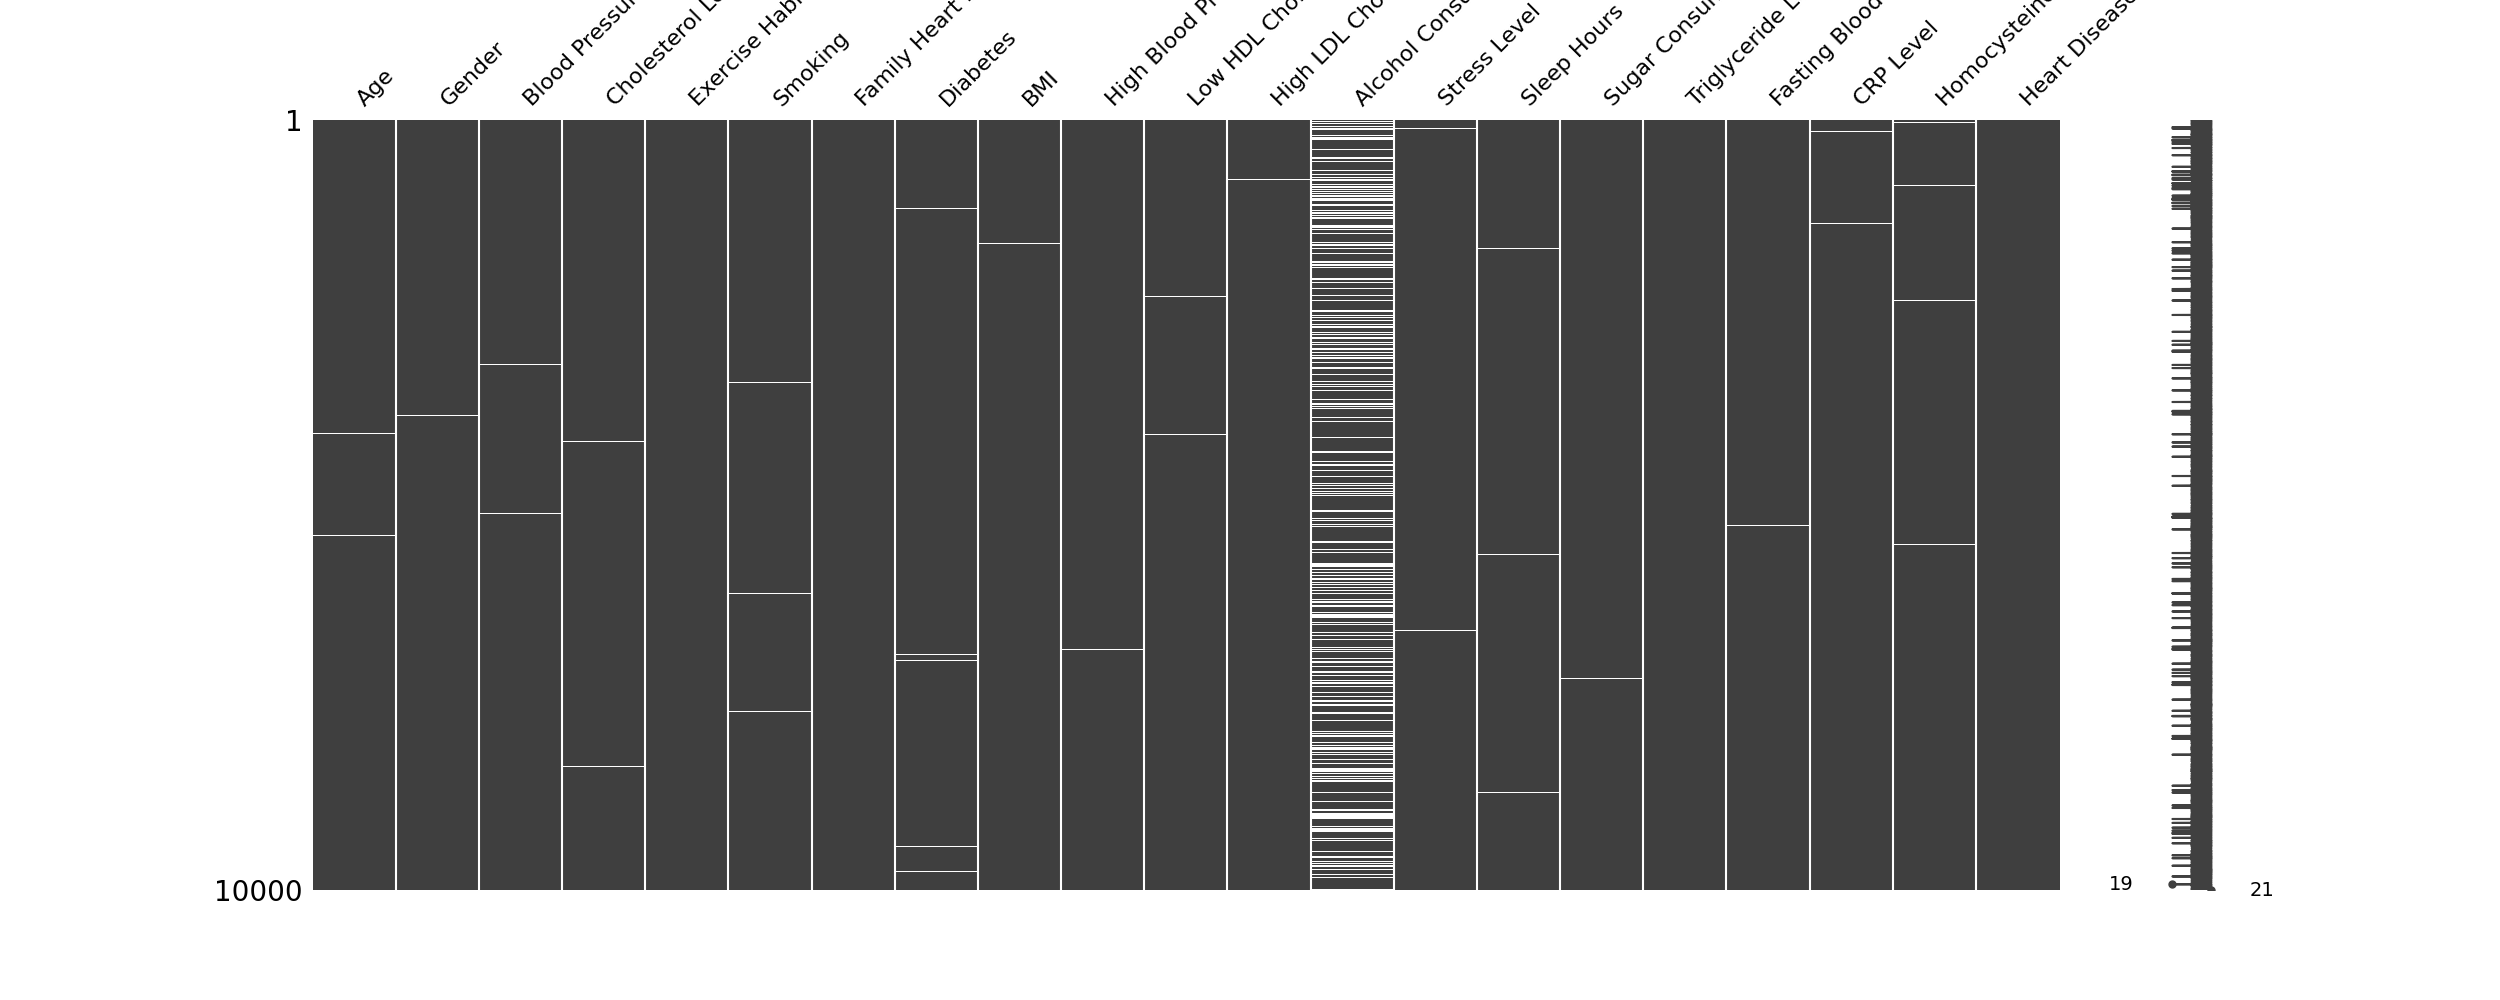
\includegraphics[width=0.8\textwidth]{./pictures/missing_values_matrix.png}
    \caption{Missing Values Matrix Visualization}
\end{figure}

% \begin{figure}[H]
%     \centering
%     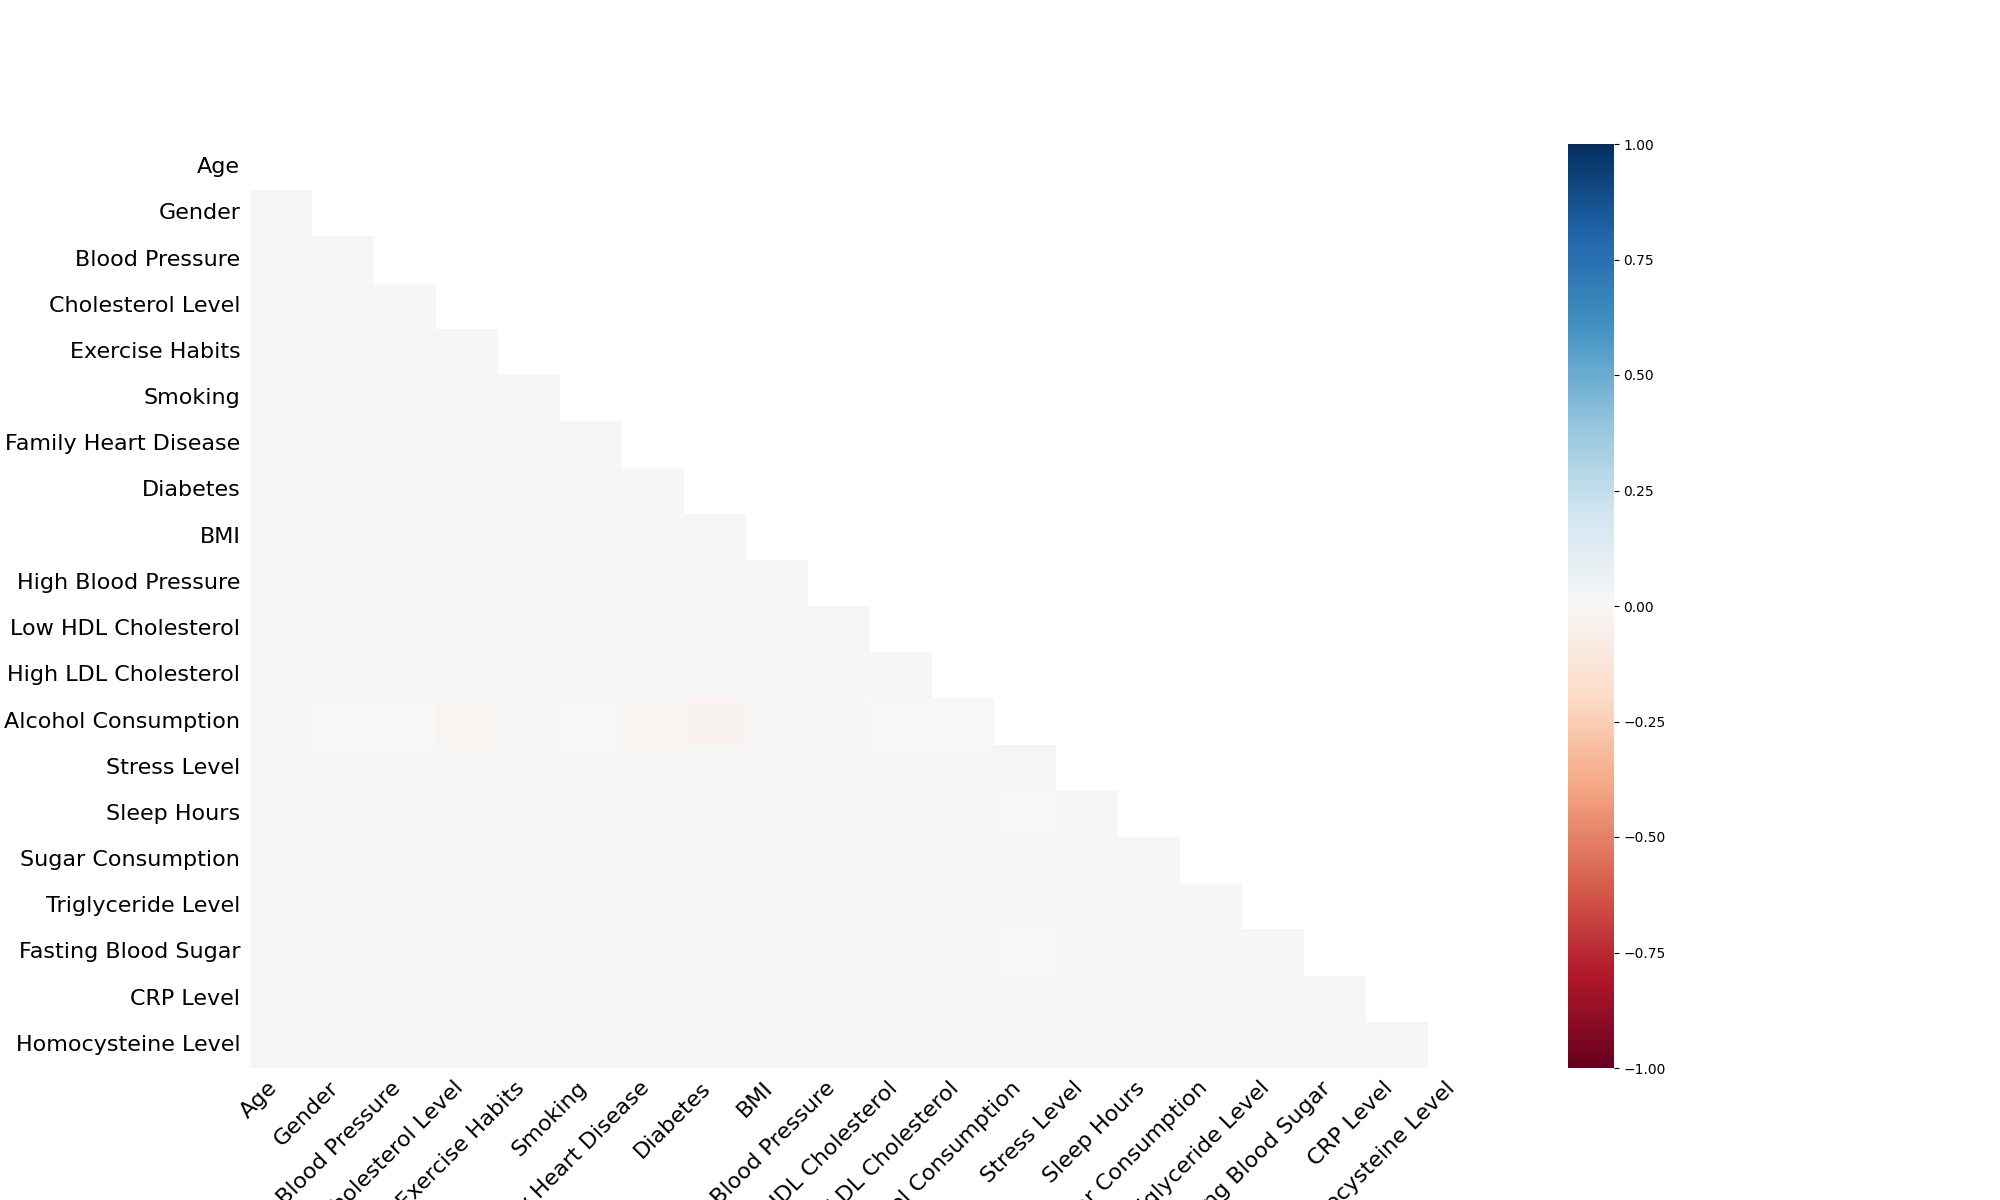
\includegraphics[width=0.8\textwidth]{./pictures/missing_values_heatmap.png}
%     \caption{Missing Values Heatmap Visualization}
% \end{figure}

The visualization above helped us identify patterns in
missing data. The matrix shows which data points are missing
across all features.

\begin{figure}[H]
    \centering
    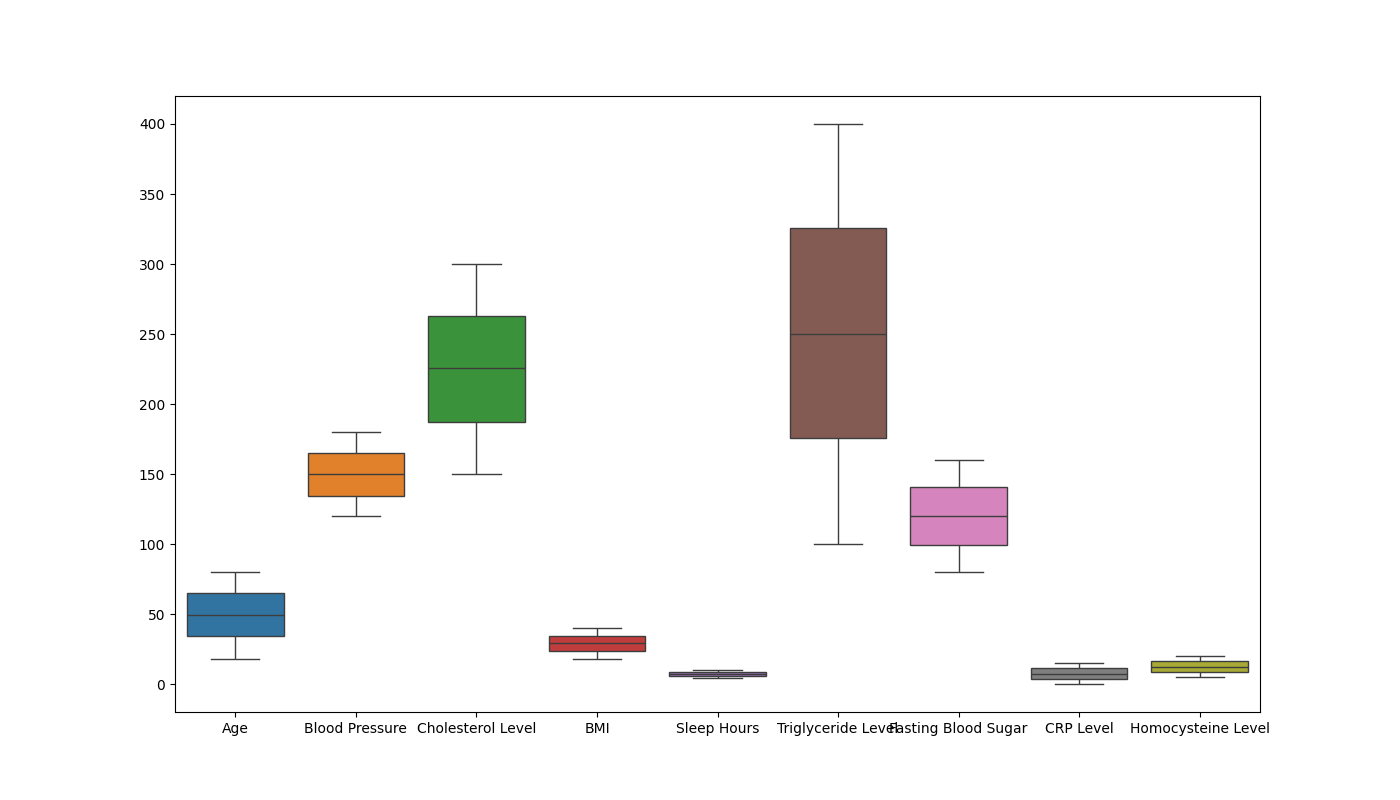
\includegraphics[width=0.8\textwidth]{./pictures/outliers.png}
    \caption{Boxplot Analysis for Outlier Detection}
\end{figure}

Our outlier analysis using boxplots showed no significant outliers in
the numerical features that would require special treatment.
This allowed us to proceed with the preprocessing without additional outlier handling steps.

Our preprocessing approach for missing values involved these steps:

\vspace{-0.25cm}
\begin{itemize}
    \vspace{-0.25cm}
    \item \textbf{Feature removal}: We completely removed the 'Alcohol Consumption' feature due to excessive missing data (25.9\%).
          \vspace{-0.25cm}
    \item \textbf{Numerical imputation}: For numerical features, we replaced missing values with column means (affecting 19-30 entries per column).
          \vspace{-0.25cm}
    \item \textbf{Categorical imputation}: For categorical features, we replaced missing values with the most frequent value (mode) in each column.
\end{itemize}

\textbf{Results}: After preprocessing, all missing values were successfully handled, creating a complete dataset with 10,000 entries and 20 features (the original 21 minus Alcohol Consumption).

\subsubsection{Feature Encoding and Transformation}
\vspace{-0.25cm}

For effective model training, we applied these transformations:

\vspace{-0.25cm}
\begin{itemize}
    \vspace{-0.25cm}
    \item \textbf{Categorical encoding}: Converted categorical variables to numerical form using one-hot encoding
          \vspace{-0.25cm}
    \item \textbf{Feature scaling}: Standardized numerical features to have zero mean and unit variance
          \vspace{-0.25cm}
    \item \textbf{Data type conversion}: Optimized data types (e.g., converted Gender to category type)
\end{itemize}
\vspace{-0.25cm}
\textbf{Results}: These transformations produced a machine learning-ready dataset with properly scaled numerical features and encoded categorical variables, enabling efficient model training.

\subsection{Methodological Challenges}

\subsubsection{Feature Selection}
\vspace{-0.25cm}
Determining the most predictive features for heart failure risk
presented a significant challenge. Through visualizations and statistical analysis, we identified several key predictors:

\begin{figure}[H]
    \centering
    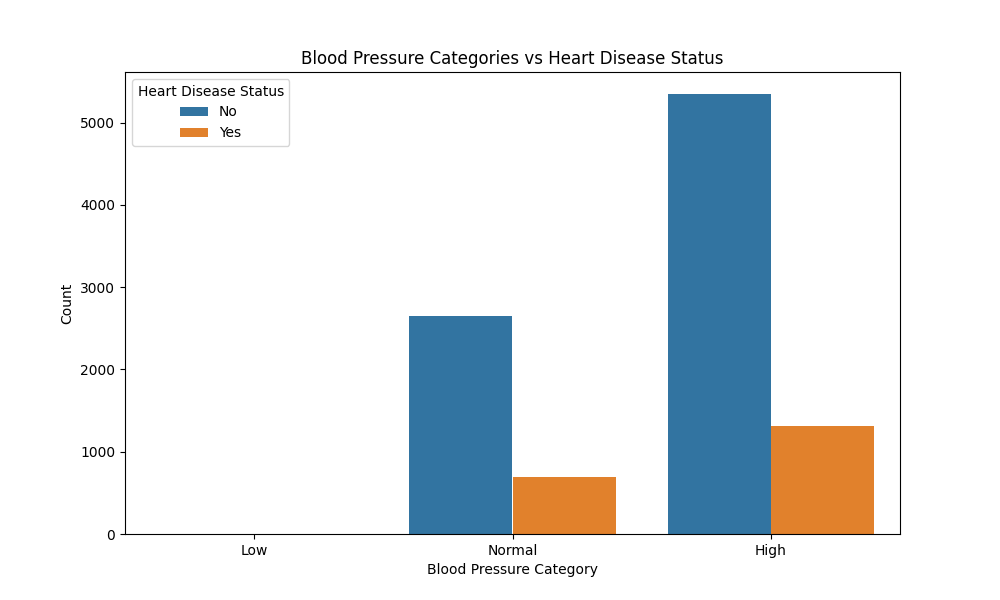
\includegraphics[width=0.8\textwidth]{./pictures/blood_pressure_categories_vs_heart_disease_status.png}
    \caption{Blood Pressure Categories vs Heart Disease Status}
\end{figure}

\textbf{Blood Pressure}: Analysis shows that individuals with higher blood pressure tend to have a higher incidence of heart disease.

\begin{figure}[H]
    \centering
    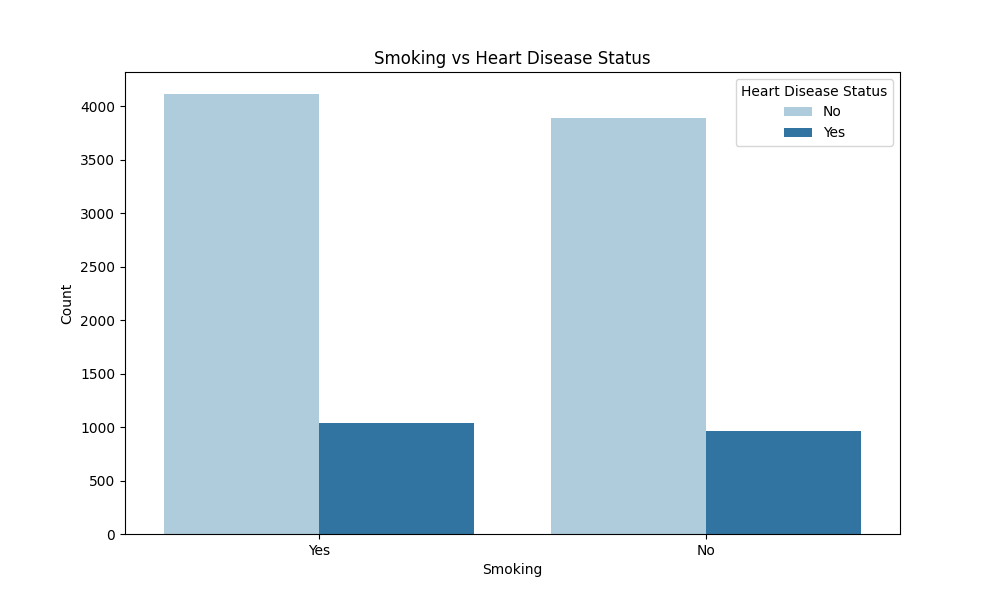
\includegraphics[width=0.8\textwidth]{./pictures/smoking_vs_heart_disease_status.png}
    \caption{Smoking vs Heart Disease Status}
\end{figure}

\textbf{Smoking}: Our visualization reveals a clear relationship between smoking habits and heart disease status.

Our initial approach included using ANOVA
F-tests to identify statistically significant features, but the
effectiveness of this method varied across different subsets
of our data.
The interrelationships between various health indicators complicated the feature
selection process, as some features that appeared
individually insignificant could become important when
considered in combination with others.

\subsubsection{Model Selection and Optimization}
\vspace{-0.25cm}
Selecting the most appropriate machine learning models for heart failure prediction required balancing accuracy, interpretability, and computational efficiency. Our project implements Neural Network and Support Vector Machine models, each presenting unique challenges:

\begin{itemize}
    \vspace{-0.25cm}
    \item \textbf{\greencheck \space Neural Network (NN)}: Our deep learning approach required careful architecture design, including determining the optimal number of hidden layers, neurons per layer, and activation functions. Additionally, preventing overfitting through techniques like dropout and early stopping required extensive experimentation.

    \item \textbf{\greencheck \space Support Vector Machine (SVM)}: While effective for high-dimensional classification, optimizing SVM required extensive hyperparameter tuning, particularly for the regularization parameter (C) and kernel selection (linear, polynomial, RBF). Finding the right balance between model complexity and generalization capability was challenging.
\end{itemize}

\subsection{Implementation Challenges}

???


\subsubsection{Data Integration}
\vspace{-0.25cm}
Working with multiple datasets from different sources
introduced integration challenges.
Variations in feature naming conventions, units of measurement,
and data collection methodologies across datasets required
careful harmonization to create a unified and consistent training dataset.

\subsubsection{Cross-Validation Strategy}
\vspace{-0.25cm}
???

% TODO: add the implementation of the models here
\section{Models Implemented}
The project implements the following machine learning models for heart
failure risk prediction:
\begin{itemize}
    \vspace{-0.25cm}
    \item \textbf{Neural Network (NN)}: A feed-forward multilayer perceptron trained on the UCI dataset with early stopping and dropout regularization.
    \item \textbf{Support Vector Machine (SVM)}: A kernelized SVM (linear and RBF kernels evaluated) optimized via grid search on the regularization parameter $C$ and kernel bandwidth.
\end{itemize}


\begin{tcolorbox}[infobox={Insights and Solutions}]
    Despite these challenges, our team implemented several effective solutions:
    \vspace{-0.25cm}
    \begin{itemize}
        \item a
        \item a
        \item a
        \item a
    \end{itemize}
\end{tcolorbox}

\section{Each Member's Implementation and Evaluation}

\subsection{Member 1 (Name, graduate/undergraduate)}

\begin{tcolorbox}[
        title=Neural Network Implementation,
        colback=lightblue!30,
        colframe=darkblue,
        boxrule=0.5pt,
        fonttitle=\bfseries\sffamily\footnotesize,
        fontupper=\footnotesize
    ]
    \textbf{Model and Implementation details:}

    The Neural Network model was implemented with the following key components:
    \begin{itemize}[leftmargin=*, itemsep=2pt, parsep=0pt]
        \item a
        \item a
        \item a
        \item a
        \item a
    \end{itemize}

    \textbf{Evaluation Results:}
    \begin{itemize}[leftmargin=*, itemsep=2pt, parsep=0pt]
        \item Accuracy:
        \item Precision:
        \item Recall:
        \item F1 Score:
        \item AUC-ROC:
    \end{itemize}
\end{tcolorbox}

\subsection{Member 2 (Name, graduate/undergraduate)}

\begin{tcolorbox}[
        title=Support Vector Machine Implementation,
        colback=lightpurple!30,
        colframe=mediumpurple,
        boxrule=0.5pt,
        fonttitle=\bfseries\sffamily\footnotesize,
        fontupper=\footnotesize
    ]
    \textbf{Model and Implementation details:}

    The SVM implementation featured:
    \begin{itemize}[leftmargin=*, itemsep=2pt, parsep=0pt]
        \item a
        \item a
        \item a
        \item a
        \item a
    \end{itemize}

    \textbf{Evaluation Results:}
    \begin{itemize}[leftmargin=*, itemsep=2pt, parsep=0pt]
        \item Accuracy:
        \item Precision:
        \item Recall:
        \item F1 Score:
        \item AUC-ROC:
    \end{itemize}
\end{tcolorbox}

\subsection{Member 3 (Name, graduate/undergraduate)}

\begin{tcolorbox}[
        title=Data Preprocessing and Feature Engineering,
        colback=lightgreen!30,
        colframe=darkgreen,
        boxrule=0.5pt,
        fonttitle=\bfseries\sffamily\footnotesize,
        fontupper=\footnotesize
    ]
    \textbf{Implementation details:}

    This work focused on:
    \begin{itemize}[leftmargin=*, itemsep=2pt, parsep=0pt]
        \item a
        \item a
        \item a
        \item a
        \item a
    \end{itemize}

    \textbf{Evaluation Results:}
    \begin{itemize}[leftmargin=*, itemsep=2pt, parsep=0pt]
        \item Accuracy:
        \item Precision:
        \item Recall:
        \item F1 Score:
        \item AUC-ROC:
    \end{itemize}
\end{tcolorbox}

\subsection{Member 4 (Name, graduate/undergraduate)}

\begin{tcolorbox}[
        title=Visualization and Model Evaluation,
        colback=mediumblue!30,
        colframe=darkblue,
        boxrule=0.5pt,
        fonttitle=\bfseries\sffamily\footnotesize,
        fontupper=\footnotesize
    ]
    \textbf{Implementation details:}

    This work focused on:
    \begin{itemize}[leftmargin=*, itemsep=2pt, parsep=0pt]
        \item a
        \item a
        \item a
        \item a
        \item a
    \end{itemize}

    \textbf{Evaluation Results:}
    \begin{itemize}[leftmargin=*, itemsep=2pt, parsep=0pt]
        \item Accuracy:
        \item Precision:
        \item Recall:
        \item F1 Score:
        \item AUC-ROC:
    \end{itemize}
\end{tcolorbox}

\end{document}